\documentclass[a4paper,10pt]{article}

% Encoding and typeface: XeLaTeX with Latin Modern Roman (fontspec default), Turkish via polyglossia
\usepackage{fontspec}
\usepackage{polyglossia}
\setdefaultlanguage{turkish}

% Layout (tight margins)
\usepackage[a4paper,top=1.2cm,bottom=1.3cm,left=1.3cm,right=1.3cm]{geometry}

% Typography
\usepackage{microtype}
\usepackage{setspace}
\setstretch{0.92}

% Paragraph settings
\setlength{\parindent}{0pt}
\setlength{\parskip}{3pt}

% Section styling
\usepackage{titlesec}
\titleformat{\section}{\bfseries\normalsize}{\thesection.}{0.4em}{}
\titlespacing*{\section}{0pt}{6pt}{3pt}

% Better lists
\usepackage{enumitem}
\setlist{noitemsep, topsep=2pt}

% Mathematics, tables, figures
\usepackage{amsmath}
\usepackage{booktabs}
\usepackage{graphicx}
\usepackage[font=small,labelfont=bf,labelsep=period,skip=3pt]{caption}
\captionsetup[figure]{name=Şekil}
\captionsetup[table]{name=Tablo}
\setlength{\textfloatsep}{8pt}
\setlength{\floatsep}{6pt}

\newcommand{\HeThreeMax}{0{,}5506}
\newcommand{\PhiZeroSixth}{0{,}0665}
\newcommand{\TThreeConst}{0{,}1100}
\newcommand{\ExpConst}{0{,}1330}
\newcommand{\ExpDThirty}{0{,}0243}
\newcommand{\LapDThirty}{0{,}00230}
\newcommand{\ExpOverLap}{10{,}6}
\newcommand{\UniDOne}{0{,}0572}
\newcommand{\ExpDOne}{0{,}159}
\newcommand{\UniRatio}{1{,}000}
\newcommand{\UniNBelow}{3}
\newcommand{\UniNLead}{3}
\newcommand{\UniDTenK}{$2{,}75\times 10^{-6}$}
\newcommand{\LapRatio}{1{,}000}
\newcommand{\LapNBelow}{7}
\newcommand{\LapNLead}{7}
\newcommand{\LapDTenK}{$6{,}88\times 10^{-6}$}
\newcommand{\TFiveRatio}{0{,}974}
\newcommand{\TFiveNBelow}{8}
\newcommand{\TFiveNLead}{14}
\newcommand{\TFiveDTenK}{$1{,}34\times 10^{-5}$}
\newcommand{\TThreeRatio}{0{,}998}
\newcommand{\TThreeNBelow}{116}
\newcommand{\TThreeNLead}{121}
\newcommand{\TThreeDTenK}{0{,}00110}
\newcommand{\ChiRatio}{1{,}000}
\newcommand{\ChiNBelow}{71}
\newcommand{\ChiNLead}{71}
\newcommand{\ChiDTenK}{$8{,}41\times 10^{-4}$}
\newcommand{\ExpRatio}{1{,}000}
\newcommand{\ExpNBelow}{177}
\newcommand{\ExpNLead}{177}
\newcommand{\ExpDTenK}{0{,}00133}
\newcommand{\LogNLead}{226}
\newcommand{\FNLead}{662}
\newcommand{\TThreeSqrtD}{0{,}1097}
\newcommand{\NoiseExact}{0{,}0193}
\newcommand{\NoiseQ}{0{,}0303}
\newcommand{\NoiseAsym}{0{,}0194}
\newcommand{\NoiseGrid}{0{,}0171}
\newcommand{\VoneNormalTenK}{0{,}0151}
\newcommand{\VoneUniTenK}{0{,}0134}
\newcommand{\VoneExpTenK}{0{,}0173}
\newcommand{\VoneUniTen}{0{,}0101}
\newcommand{\UniDTen}{0{,}00281}
\newcommand{\NormalFramesBelow}{30}
\newcommand{\UniFramesBelow}{30}
\newcommand{\LapFramesBelow}{30}
\newcommand{\TFiveFramesBelow}{30}
\newcommand{\ChiFramesBelow}{26}
\newcommand{\ExpFramesBelow}{22}
\newcommand{\ExpNoiseN}{48}
\newcommand{\UniNoiseN}{2}
\newcommand{\ParetoFramesCut}{19}
\newcommand{\ParetoMaxKs}{0{,}151}
\newcommand{\FFramesCut}{2}
\newcommand{\RUniThirty}{8{,}8\times 10^{5}}
\newcommand{\RUniThousand}{1{,}0\times 10^{9}}
\newcommand{\RExpThirty}{1.279}
\newcommand{\RExpThousand}{42.676}
\newcommand{\RTThreeThousand}{63.293}
\newcommand{\IqrSlopeParetoTwoFive}{-0{,}46}
\newcommand{\IqrSlopeParetoOneFive}{-0{,}30}
\newcommand{\IqrSlopeCauchy}{-0{,}006}
\newcommand{\CauchyIqrOne}{1{,}98}
\newcommand{\CauchyIqrTenK}{2{,}01}
\newcommand{\ParetoSlope}{-0{,}23}
\newcommand{\ParetoTen}{0{,}152}
\newcommand{\ParetoHundred}{0{,}085}
\newcommand{\ParetoThousand}{0{,}049}
\newcommand{\ParetoTenK}{0{,}031}
\newcommand{\LogSlope}{-0{,}42}
\newcommand{\FSlope}{-0{,}40}
\newcommand{\LogSimTen}{0{,}045}
\newcommand{\LogLeadTen}{0{,}048}
\newcommand{\FSimTen}{0{,}061}
\newcommand{\FLeadTen}{0{,}081}
\newcommand{\NoiseHundredK}{0{,}0027}


\begin{document}

% Header (top-right)
\begin{flushright}
\small \textbf{Derlenme tarihi:} \today
\end{flushright}

\vspace{-6pt}
\hrule
\vspace{24pt}

\textbf{BAŞLIK:} Merkezî limit teoremi ne kadar hızlı işler? Kesin uzaklıklar, benzetim gürültüsü ve kalın kuyruklar

\textbf{KONU:} \texttt{CLT-speed-race-exercise} deposunun 2.\ sürümündeki analizlerin amacı, yöntemi ve sonuçları

\textbf{HAZIRLAYAN:} Muhammed İkbal Yılmaz (myucanlar@gmail.com)

\vspace{12pt}

\section{Amaç ve kapsam}

$X_1, X_2, \dots$ ortalaması $\mu$, varyansı $\sigma^2$ olan bir dağılımdan bağımsız çekilişler olsun ve
$Z_n = \sqrt n\,(\bar X_n - \mu)/\sigma$, dağılım fonksiyonu $F_n$ olan standartlaştırılmış örneklem ortalaması olsun.
$0 < \sigma^2 < \infty$ ise merkezî limit teoremi (MLT) her $x$ için $F_n(x) \to \Phi(x)$ olduğunu söyler. Bunun ne kadar hızlı
gerçekleştiği burada Kolmogorov uzaklığıyla ölçülür:
\[
D_n = \sup_x \lvert F_n(x) - \Phi(x)\rvert ,
\]
yani normal yaklaşımla hesaplanan herhangi bir $P(Z_n \le x)$ olasılığındaki en büyük hata. Projenin 1.\ sürümü on dağılım için
$Z_n$'nin $R = 2000$ tekrarlı benzetimlerini canlandırmış ve dağılımları göz kararıyla gruplamıştı: hızlı (Normal, Tekdüze), daha
yavaş (Üstel, Laplace), çok yavaş (az serbestlik dereceli Student-t) ve başarısız (kuyruk indeksi $\le 2$ olan Pareto, Cauchy). Bu
not üç soru sorar:

\begin{enumerate}
  \item \textbf{$D_n$ tam olarak ne kadardır ve azalma hızını ne belirler?} Dağılımlardan altısı kesin hesaba izin verir.
  \item \textbf{$R = 2000$ tekrarlı bir benzetim neyi ölçebilir?} Tam olarak normal olan bir $Z_n$ bile sıfırdan büyük bir benzetim
  uzaklığı verir.
  \item \textbf{Geri kalan dağılımlarda ne olur:} burada kesin yöntemi olmayan Lognormal, F ve Pareto ile 1.\ sürümün durduğu,
  varyansı sonsuz olan Cauchy ve Pareto?
\end{enumerate}

Tüm dağılımlar 1.\ sürümün varsayılan parametrelerini kullanır: Tekdüze(0, 1), Üstel(1), Laplace(0, 1), $\sigma = 0{,}6$ olan
Lognormal, Ki-kare(5), F(5, 10), Student-t(5), kuyruk indeksi 2,5 olan Pareto. Varyansı sonlu olan en küçük tamsayı serbestlik
derecesi olarak Student-t(3) eklenmiştir.

\section{Yöntem}

\begin{itemize}
  \item \textbf{Kesin uzaklıklar.} Üstel ve Ki-kare dağılımlarında $n$ çekilişin toplamı gama dağılımlıdır; dolayısıyla $F_n$ düzenli
  eksik gama fonksiyonudur. $n \le 40$ için Tekdüze dağılımda toplam Irwin--Hall dağılımına uyar ve kesin rasyonel aritmetikle
  hesaplanır. Diğer durumlarda (Laplace, $n > 40$ için Tekdüze, Student-t) $F_n - \Phi$, iki karakteristik fonksiyonun farkı Gil-Pelaez
  (1951) formülü ve Gauss--Legendre kareleme yöntemiyle ters çevrilerek elde edilir. Bu ters çevirme, kesin yöntemlerle ve Laplace
  ($n = 2$) ile Student-t ($n = 1$) için kapalı formlarla $3\times 10^{-15}$ içinde örtüşür. Supremum, $[-8, 8]$ üzerinde $0{,}02$
  adımlı bir ızgarada bulunur ve sayısal olarak inceltilir.
  \item \textbf{Öncü terimler.} Dördüncü momenti sonlu sürekli bir dağılım için Edgeworth açılımı (Hall, 1992)
  $F_n(x) - \Phi(x) = -\varphi(x)\bigl[\tfrac{\gamma}{6\sqrt n}He_2(x) + \tfrac{\kappa_4}{24n}He_3(x) + \tfrac{\gamma^2}{72n}He_5(x)\bigr]
  + o(1/n)$ verir; $\gamma$ çarpıklık, $\kappa_4$ fazla basıklık, $He_k$ Hermite polinomlarıdır. $\gamma \ne 0$ ise $D_n$'nin öncü
  terimi $\lvert\gamma\rvert\varphi(0)/(6\sqrt n) = \PhiZeroSixth\,\lvert\gamma\rvert/\sqrt n$, $\gamma = 0$ ise
  $\lvert\kappa_4\rvert \cdot \HeThreeMax/(24n)$'dir; burada $\HeThreeMax = \max_x\lvert He_3(x)\varphi(x)\rvert$. Student-t(3)'ün
  üçüncü mutlak momenti sonlu değildir. Standartlaştırılmış karakteristik fonksiyonu $(1+\lvert s\rvert)e^{-\lvert s\rvert} = 1 - s^2/2 +
  \lvert s\rvert^3/3 + O(s^4)$'tür ve $\lvert s\rvert^3/3$ terimi $\TThreeConst/\sqrt n$ öncü terimini verir (bu not için türetilmiş ve
  sayısal olarak hesaplanmıştır).
  \item \textbf{Benzetim.} 1.\ sürümün benzetimi çekiliş çekiliş yinelenir (aynı tohum, rastgele sayı üretecinin aynı çağrıları); 1.\
  sürümün kaydettiği karelerde yazan dört uzaklığı aynen verir. Bir benzetimin gürültüsü, gerçek dağılımdan $R$ çekilişin Kolmogorov
  istatistiğiyle ölçülür; bu istatistiğin kesin dağılımı SciPy'da (\texttt{scipy.stats.kstwo}) bulunur.
  \item \textbf{Denetimler.} On yedi birim testi kodu bağımsız hesaplarla karşılaştırır: momentleri SciPy ile, karakteristik
  fonksiyonları yoğunlukların sayısal Fourier integralleriyle, ters çevirmeyi kesin dağılım fonksiyonlarıyla, supremumu kaba kuvvet
  aramasıyla.
\end{itemize}

\section{Analiz 1: Yakınsamanın kesin hızı (Şekil~\ref{fig:exact}, Tablo~\ref{tab:summary})}

\textbf{Neden.} Göz kararıyla yapılan bir sıralama, bir dağılımın diğerinden ne kadar hızlı yakınsadığını ya da nedenini söyleyemez.
Kesin $D_n$ ilk soruyu, öncü terimlerle karşılaştırma ise ikincisini yanıtlar.

\textbf{Yöntem.} Altı dağılım için 1 ile $10^4$ arasında logaritmik ölçekte eşit aralıklı 41 $n$ değerinde $D_n$. Her biri için
$D_n < 0{,}01$ olan en küçük $n$; bu değere kadar her $n$ için $D_n$ hesaplanarak ve sonraki 200 değer denetlenerek bulunmuştur.

\textbf{Şekil nasıl okunmalı.} Solda: iki eksen de logaritmiktir; $n^{-1/2}$ ile orantılı bir uzaklık $-1/2$, $n^{-1}$ ile orantılı
olan $-1$ eğimli bir doğrudur. Kesikli çizgiler öncü terimlerdir. Sağda: $D_n$'nin öncü terimine oranı; 1'e yaklaşan bir eğri,
yakınsama hızını öncü terimin açıkladığı anlamına gelir.

\begin{figure}[h]
\centering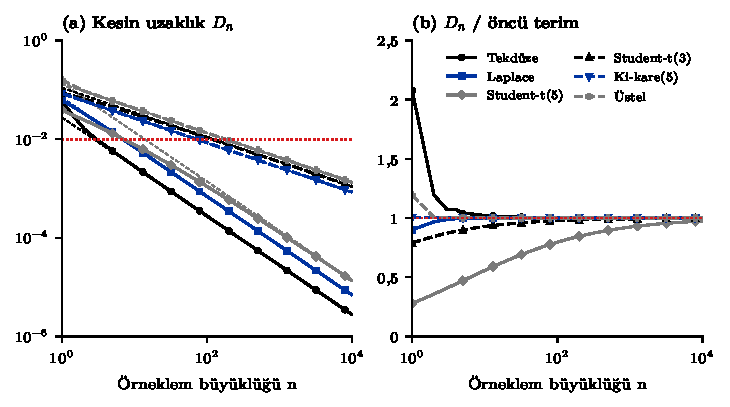
\includegraphics[width=0.9\linewidth]{../figures/tr/fig1_exact_speed.pdf}
\caption{Standartlaştırılmış ortalama ile normal dağılım arasındaki kesin Kolmogorov uzaklığı. Solda: $D_n$ (düz) ve öncü terimi
(kesikli); noktalı: $0{,}01$. Sağda: $D_n$'nin öncü terimine oranı.}\label{fig:exact}
\end{figure}

\begin{table}[h]
\centering\footnotesize
\caption{Çarpıklık $\gamma$, fazla basıklık $\kappa_4$, $D_n$'nin öncü terimi, kesin $D_n$ ve $D_n < 0{,}01$ olan en küçük $n$: kesin
ve öncü terimin öngördüğü. --: mevcut değil ya da burada kesin yöntem yok.}\label{tab:summary}
\begin{tabular}{lrrrrrrr}
\toprule
Dağılım & $\gamma$ & $\kappa_4$ & Öncü terim & $D_{30}$ & $D_{1000}$ & $D_n<0{,}01$ için $n$ & öncü terime göre \\
\midrule
Normal & 0 & $0$ & 0 & 0 & 0 & 1 & -- \\
Tekdüze & 0 & $-1{,}20$ & $0{,}0275\,n^{-1}$ & $9{,}24\times 10^{-4}$ & $2{,}75\times 10^{-5}$ & 3 & 3 \\
Laplace & 0 & $3{,}00$ & $0{,}0688\,n^{-1}$ & 0{,}00230 & $6{,}88\times 10^{-5}$ & 7 & 7 \\
Student-t(5) & 0 & $6{,}00$ & $0{,}1376\,n^{-1}$ & 0{,}00314 & $1{,}27\times 10^{-4}$ & 8 & 14 \\
Student-t(3) & -- & -- & $0{,}1100\,n^{-1/2}$ & 0{,}0192 & 0{,}00345 & 116 & 121 \\
Ki-kare(5) & 1{,}26 & $2{,}40$ & $0{,}0841\,n^{-1/2}$ & 0{,}0154 & 0{,}00266 & 71 & 71 \\
Üstel & 2{,}00 & $6{,}00$ & $0{,}1330\,n^{-1/2}$ & 0{,}0243 & 0{,}00421 & 177 & 177 \\
Lognormal(0,6) & 2{,}26 & $10{,}3$ & $0{,}1503\,n^{-1/2}$ & -- & -- & -- & 226 \\
F(5, 10) & 3{,}87 & $50{,}9$ & $0{,}2571\,n^{-1/2}$ & -- & -- & -- & 662 \\
Pareto(2,5) & -- & -- & -- & -- & -- & -- & -- \\
Cauchy & \multicolumn{7}{l}{ortalama ve varyans yok} \\
\bottomrule

\end{tabular}
\end{table}

\textbf{Bulgu.} Dağılımlar iki gruba ayrılır. Dördüncü momenti sonlu simetrik dağılımlarda (Tekdüze, Laplace, Student-t(5)) $D_n$,
$1/n$ gibi; çarpık olanlarda (Ki-kare(5), Üstel) yalnızca $1/\sqrt n$ gibi azalır. Student-t(3) simetrik olduğu hâlde o da
$1/\sqrt n$ gibi azalır. $n = 10^4$'te öncü terime oran Tekdüze için \UniRatio{}, Laplace için \LapRatio{}, Ki-kare için \ChiRatio{},
Üstel için \ExpRatio{}, Student-t(3) için \TThreeRatio{}'dir; Student-t(5) için 1'e daha yavaş yaklaşır (\TFiveRatio{}). Öncü terim,
$D_n < 0{,}01$ olan en küçük $n$'yi Tekdüze, Laplace, Ki-kare ve Üstel için tam olarak öngörür (sırasıyla $n = \UniNBelow$, $\LapNBelow$,
$\ChiNBelow$, $\ExpNBelow$). Lognormal(0,6) ve F(5, 10) için öngörüsü yaklaşık $n = \LogNLead$ ve $\FNLead$ biçimindedir. $n = 30$'da
Üstel hâlâ $D_{30} = \ExpDThirty$ düzeyindedir; bu, Laplace'ın ($\LapDThirty$) \ExpOverLap{} katıdır.

\textbf{Yorum.} Yakınsama hızını esas olarak çarpıklık belirler: hatanın $1/\sqrt n$ gibi mi yoksa $1/n$ gibi mi azalacağına o karar
verir. Dördüncü moment sonlu kaldıkça kuyrukların kalınlığı tek başına hızı değiştirmez: Laplace'ın kuyrukları tekdüze dağılımınkinden
kalındır, ama aynı hızla yakınsar; 1.\ sürüm onu yanlışlıkla Üstel'in yanına koymuştu. Student-t(3)'ü yavaşlatan, çarpıklık olmadan
bir $1/\sqrt n$ terimi ekleyen sonsuz üçüncü mutlak momenttir; 1.\ sürümün varsayılanı olan Student-t(5) ise $n = \TFiveNBelow$'de
$D_n < 0{,}01$ düzeyine ulaşır. ``$n \ge 30$'' gibi tek bir kural bunu anlatamaz: 1.\ sürümün dağılımları arasında $D_n < 0{,}01$ için
gereken $n$, $\UniNBelow$ (Tekdüze) ile yaklaşık $\FNLead$ (F(5, 10), öncü terim tahmini) arasında değişir ve Pareto(2,5) $n = 10^4$'te
bile bu düzeye ulaşmamıştır (analiz 3).

\section{Analiz 2: 2000 tekrarlı bir benzetim neyi ölçer (Şekil~\ref{fig:mc})}

\textbf{Neden.} 1.\ sürüm uzaklığı $Z_n$'nin benzetimle elde edilen $R = 2000$ değerinden, $[-12, 12]$ üzerindeki 401 ızgara
noktasında $\max\lvert\hat F(x) - \Phi(x)\rvert$ olarak ölçmüştü. $R$ sonlu olduğundan, $F_n = \Phi$ olduğunda bile $\hat F$, $F_n$'den
farklıdır. Benzetim uzaklığı yakınsamayı ancak $D_n$ bu gürültünün üzerinde olduğu sürece gösterebilir.

\textbf{Yöntem.} Normal, Tekdüze ve Üstel için 1.\ sürümün benzetimi (tohum 42, 10 ile $10^4$ arasında 30 örneklem büyüklüğü), kesin
$D_n$ ile karşılaştırılır. $R = 2000$ için ortalama gürültü, kesin ampirik uzaklık için \NoiseExact{} (\%95 kantil \NoiseQ{}; asimptotik
değer $\sqrt{\pi/2}\,\ln 2/\sqrt R = \NoiseAsym$), 1.\ sürümün ızgara uzaklığı için \NoiseGrid{}'dir (400 benzetilmiş örneklem). Sağ
panel: ortalama gürültünün, $0{,}8687/\sqrt R$, $D_n$'ye eşit olduğu tekrar sayısı.

\textbf{Şekil nasıl okunmalı.} Solda: işaretler 1.\ sürümün uzaklıkları, çizgiler kesin $D_n$'dir; gölgeli bölge ortalama gürültünün
altında kalır. Sağda: noktalı çizgiler 1.\ sürümün sunduğu varsayılan ve en büyük $R$'yi gösterir.

\begin{figure}[h]
\centering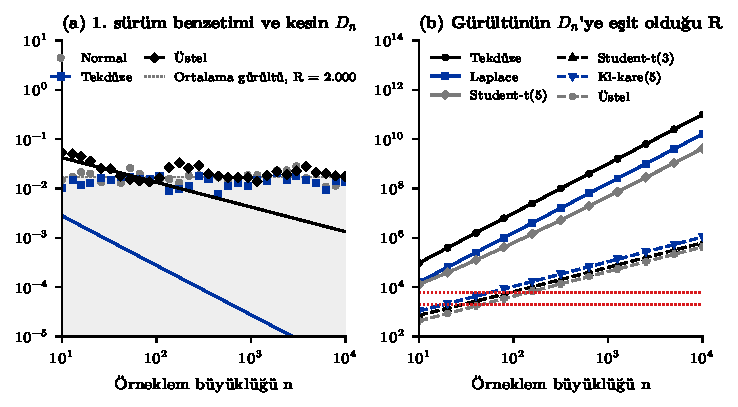
\includegraphics[width=0.9\linewidth]{../figures/tr/fig2_monte_carlo.pdf}
\caption{Solda: 1.\ sürümün benzetim uzaklıkları (işaretler; $R = 2000$, tohum 42) ve kesin $D_n$ (çizgiler); noktalı: 1.\ sürümün ızgara
uzaklığının ortalama gürültüsü. Sağda: ortalama gürültünün $D_n$'ye eşit olması için gereken tekrar sayısı.}\label{fig:mc}
\end{figure}

\textbf{Bulgu.} Normal dağılımda $Z_n$ tam olarak normaldir; yine de 1.\ sürüm $n = 10^4$'te \VoneNormalTenK{} bildirir. Tekdüze için
\VoneUniTenK{} bildirir; kesin uzaklık ise yalnızca \UniDTenK{} düzeyindedir. Kesin uzaklık, kesin ampirik uzaklığın ortalama gürültüsünün
(\NoiseExact{}) altına Üstel için $n = \ExpNoiseN$'den, Tekdüze için $n = \UniNoiseN$'den itibaren iner. Her çalıştırmanın 30 karesinden
kesin uzaklığın 1.\ sürümün gürültüsünün altında olduğu kare sayısı Tekdüze, Laplace ve Student-t(5) için \UniFramesBelow{}, Ki-kare(5)
için \ChiFramesBelow{}, Üstel için \ExpFramesBelow{}'dir. Ortalama gürültüyü $D_n$ kadar küçültmek için Tekdüze'de $n = 30$'da
$R \approx \RUniThirty$, $n = 1000$'de $\RUniThousand$ tekrar gerekir; Üstel'de bu sayılar sırasıyla $\RExpThirty$ ve $\RExpThousand$ olur. 1.\
sürüm $\hat F - \Phi$ farkını yaklaşık $\pm 0{,}055$ sabit sınırlarla da çizmişti; Pareto(2,5) için uzaklık 30 karenin
\ParetoFramesCut{}'unda bu sınırları aştı (\ParetoMaxKs{}'e kadar).

\textbf{Yorum.} 1.\ sürümdeki yarışın karelerinin çoğu yakınsamayı değil, benzetim gürültüsünü gösterir: birkaç düzine çekilişten
sonra Pareto(2,5) dışındaki her dağılım normale eşit derecede yakın görünür. Bir benzetim ancak yaklaşık $0{,}87/\sqrt R$'den büyük
uzaklıkları ayırt edebilir; simetrik dağılımlar arasındaki farklar orta büyüklükteki $n$'lerde milyonlarca ile milyarlarca tekrar
gerektirir. Bunları karşılaştırmanın tek pratik yolu kesin hesaptır.

\section{Analiz 3: Kalın kuyruklar (Şekil~\ref{fig:heavy})}

\textbf{Neden.} 1.\ sürümden iki soru kalır: burada kesin yöntemi olmayan Lognormal, F ve Pareto(2,5) ne kadar hızlı yakınsar; ve
1.\ sürümün yalnızca bir ileti yazdırdığı sonsuz varyans durumunda örneklem ortalaması ne yapar?

\textbf{Yöntem.} (a) Sonlu varyans olmadan da var olan $\bar X_n$'nin çeyrekler açıklığı (ÇAA): kuyruk indeksi 2,5 ve 1,5 olan Pareto
ile Cauchy, $n$ 1'den $10^4$'e, $R = 20.000$ yol (Pareto(2,5) için $100.000$); karşılaştırma için Normal(0, 1)'in kesin ÇAA'sı
$2 \cdot 0{,}6745/\sqrt n$. (b) Lognormal(0,6), F(5, 10) ve Pareto(2,5) için $R = 100.000$ yolla $Z_n$'nin benzetim uzaklığı
(ortalama gürültü \NoiseHundredK{}). Eğimler log--log ölçekte, $n \ge 10$ için ve benzetim uzaklığının gürültünün üç katını aştığı
yerlerde uydurulur.

\textbf{Şekil nasıl okunmalı.} İki panel de logaritmiktir. Solda: $-1/2$ eğimi MLT'nin $1/\sqrt n$ hızındaki daralmasıdır; yatay bir
çizgi, ortalama almanın yayılımı azaltmadığı anlamına gelir. Sağda: kesikli çizgiler, çarpıklığın var olduğu yerlerde öncü terimlerdir.

\begin{figure}[h]
\centering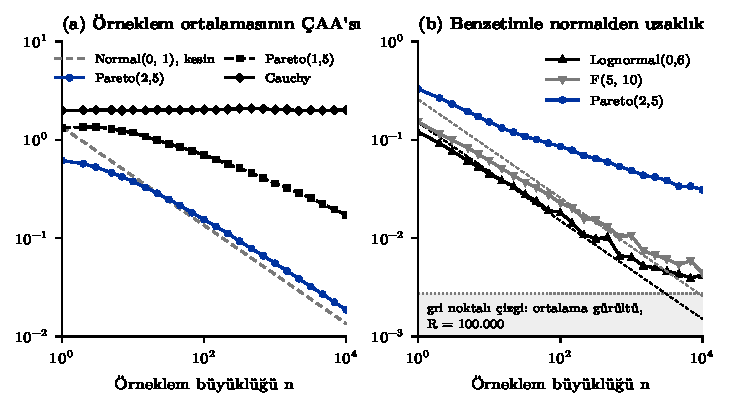
\includegraphics[width=0.9\linewidth]{../figures/tr/fig3_heavy_tails.pdf}
\caption{Solda: örneklem ortalamasının ÇAA'sı. Sağda: $Z_n$'nin normal dağılıma benzetim uzaklığı ($R = 100.000$) ve öncü terimler
(kesikli); gölgeli: ortalama gürültünün altı.}\label{fig:heavy}
\end{figure}

\textbf{Bulgu.} Cauchy ortalamasının ÇAA'sı $n = 1$'de \CauchyIqrOne{}, $n = 10^4$'te \CauchyIqrTenK{}'dir (eğim $\IqrSlopeCauchy$):
$n$ Cauchy değişkeninin ortalaması tek bir değişkenle aynı Cauchy dağılımına sahiptir. Ortalaması olan ama varyansı olmayan Pareto(1,5)
için $n \ge 100$'de eğim $\IqrSlopeParetoOneFive$'dur; bu, genelleştirilmiş MLT'nin verdiği $1/\alpha - 1 = -1/3$ değerine yakındır
(Gnedenko ve Kolmogorov, 1954). Pareto(2,5) için eğim $\IqrSlopeParetoTwoFive$'dır ve hâlâ $-1/2$'ye yaklaşmaktadır. Lognormal(0,6) ve
F(5, 10) için benzetim uzaklığı $\LogSlope$ ve $\FSlope$ eğimleriyle azalır; $n = 10$'da öncü terime karşılık değerler Lognormal için
\LogSimTen{} ve \LogLeadTen{}, F için \FSimTen{} ve \FLeadTen{}'dir. Üçüncü momenti sonsuz olan Pareto(2,5) çok daha yavaş yakınsar:
$n = 10$, $10^2$, $10^3$, $10^4$ için \ParetoTen{}, \ParetoHundred{}, \ParetoThousand{} ve \ParetoTenK{} (eğim $\ParetoSlope$).
$n = 10^4$'te normalden uzaklığı, Üstel'in $n = 30$'daki uzaklığından fazladır.

\textbf{Yorum.} Varyans sonsuz olduğunda örneklem ortalamasının yayılımı $1/\sqrt n$ gibi daralmaz. Cauchy'de ortalama almak yayılımı
hiç azaltmaz. Pareto(1,5)'te ortalama yine $\mu$'ye yakınsar, ama $n^{1/\alpha - 1}$ hızıyla ve normal olmayan (kararlı) bir limite;
bu yüzden $\sqrt n$ ile standartlaştırılmış bir histogram oturamaz. Sonlu varyans tek başına yakınsamayı güvence altına alır, hızını
değil. Lyapunov--Katz sınırı (Katz, 1963) $D_n \le C\,\nu_{2+\delta}\, n^{-\delta/2}$, $0 < \delta \le 1$, der; burada
$\nu_{2+\delta} = E\lvert Y\rvert^{2+\delta}$, $Y$ standartlaştırılmış değişkendir. Pareto(2,5)'te yalnızca 2,5'ten küçük mertebeden
momentler vardır; dolayısıyla sınır yalnızca $\delta < 0{,}5$ ile uygulanır ve en fazla yaklaşık $n^{-1/4}$ hızında bir azalmayı
güvenceler. Ölçülen eğim, $\ParetoSlope$, bu mertebededir.

\section{Sonuçlar ve sınırlılıklar}

\begin{itemize}
  \item Yakınsama hızını esas olarak çarpıklık belirler: dördüncü momenti sonlu simetrik dağılımlarda $D_n$, $1/n$ gibi, çarpık
  dağılımlarda $1/\sqrt n$ gibi azalır; sabiti Edgeworth açılımının öncü terimi verir. Sonsuz üçüncü momentler (Student-t(3),
  Pareto(2,5)) yakınsamayı daha da yavaşlatır.
  \item $R$ tekrarlı bir benzetim yaklaşık $0{,}87/\sqrt R$'nin altındaki uzaklıkları ayırt edemez. 1.\ sürümdeki yarışın karelerinin
  çoğu bu gürültüyü gösterir.
  \item Varyans sonsuz olduğunda MLT olağan biçimiyle geçerli değildir: Cauchy ortalaması yoğunlaşmaz, Pareto(1,5) ortalaması
  $n^{-1/3}$ gibi yoğunlaşır.
  \item Kolmogorov uzaklığı bir olasılıktaki en büyük hatayı ölçer; kuyruklardaki göreli hatayı ölçmez, bu çok daha büyük olabilir.
  Lognormal, F ve Pareto yalnızca benzetimle incelenmiştir. Yalnızca 1.\ sürümün varsayılan parametreleri kullanılmıştır.
\end{itemize}

\section*{Kaynaklar}
{\small
Gil-Pelaez, J. (1951). Note on the inversion theorem. \textit{Biometrika}, 38(3--4), 481--482.\\
Gnedenko, B. V., Kolmogorov, A. N. (1954). \textit{Limit Distributions for Sums of Independent Random Variables}. Addison-Wesley.\\
Hall, P. (1992). \textit{The Bootstrap and Edgeworth Expansion}. Springer.\\
Katz, M. L. (1963). Note on the Berry--Esseen theorem. \textit{Annals of Mathematical Statistics}, 34(3), 1107--1108.\\
SciPy belgeleri: \texttt{scipy.special.gammainc}, \texttt{scipy.stats.kstwo}.

\smallskip
Kodun yazımında ve bu notun hazırlanmasında bir yapay zekâ kodlama asistanından yararlanılmıştır. Tüm sayılar
\texttt{figures/*.csv} dosyalarından \texttt{make\_paper.py} ile üretilmiştir.
}

\end{document}
